\documentclass[12pt,a4paper]{scrartcl}

\author{Sebastian Hirnschall}
%% (C) Hirnschall Sebastian 2016 
\date{\today}


\usepackage[
backend=biber,
style=authoryear-icomp,    % Zitierstil
isbn=false,                % ISBN nicht anzeigen, gleiches geht mit nahezu allen anderen Feldern
pagetracker=true,          % ebd. bei wiederholten Angaben (false=ausgeschaltet, page=Seite, spread=Doppelseite, true=automatisch)
maxbibnames=50,            % maximale Namen, die im Literaturverzeichnis angezeigt werden (ich wollte alle)
maxcitenames=3,            % maximale Namen, die im Text angezeigt werden, ab 4 wird u.a. nach den ersten Autor angezeigt
autocite=inline,           % regelt Aussehen für \autocite (inline=\parancite)
block=space,               % kleiner horizontaler Platz zwischen den Feldern
backref=true,              % Seiten anzeigen, auf denen die Referenz vorkommt
backrefstyle=three+,       % fasst Seiten zusammen, z.B. S. 2f, 6ff, 7-10
date=short                % Datumsformat
]{biblatex}

\addbibresource{refs.bib}

\usepackage{longtable}
%\usepackage{hyperref}
\usepackage{amsmath}% http://ctan.org/pkg/amsmath
\usepackage[english]{cleveref} %referenzen fur Abbildungen
\usepackage{graphicx}
\usepackage{listings}
\usepackage{esdiff}
\usepackage[utf8]{inputenc}
\usepackage[english]{babel}
\usepackage[T1]{fontenc}
\usepackage{graphicx}
\usepackage{amssymb}
\usepackage{geometry}% http://ctan.org/pkg/geometry
\usepackage{amsthm}
\usepackage{tocloft}
\usepackage{framed}
\usepackage{mathtools}
\usepackage{color}
\usepackage{multirow}
\usepackage{textcomp}
\usepackage{subcaption}
\usepackage{float}
%\usepackage[dvipsnames]{xcolor}
\usepackage[ruled,vlined]{algorithm2e}



\usepackage[table,xcdraw,dvipsnames]{xcolor}

\usepackage{fancyvrb}

\usepackage{tikz}
\usetikzlibrary{spy}
\usetikzlibrary{calc,arrows}

% redefine \VerbatimInput
\RecustomVerbatimCommand{\VerbatimInput}{VerbatimInput}%
{fontsize=\footnotesize,
	%
	frame=lines,  % top and bottom rule only
	framesep=2em, % separation between frame and text
	rulecolor=\color{Gray},
	%
	label=\fbox{\color{Black}yahoo-stats.txt},
	labelposition=topline,
	%
}


%change title font
%\usepackage{titlesec}
%\setkomafont{\section}{\LARGE\bfseries}
%\setkomafont{\subsection}{\Large\bfseries}
%\setkomafont{\subsubsection}{\large\bfseries}
%\setkomafont{\paragraph}{\large\bfseries}
%\setkomafont{\subparagraph}{\large\bfseries}




%\pagestyle{headings}

\setcounter{secnumdepth}{5}
\setcounter{tocdepth}{5}

%\pagestyle{headings}

\usepackage{fancyhdr}
\pagestyle{fancy}
%
\rhead{ \rightmark}
%\rhead[re]{\textbf{\nouppercase{\leftmark}}}
\chead{}
\lhead{}
%%
\lfoot{Sebastian Hirnschall}
\cfoot{}
\rfoot{\thepage}
%%
\renewcommand{\headrulewidth}{0.2pt}
\renewcommand{\footrulewidth}{0.2pt}


\fancypagestyle{firststyle}
{
	\fancyhf{}
	\rhead{}
	%\rhead[re]{\textbf{\nouppercase{\leftmark}}}
	\chead{}
	\lhead{}
	\lfoot{ Sebastian Hirnschall}
	\cfoot{}
	\rfoot{\thepage}
}


%listings settings
\definecolor{mygreen}{rgb}{0,0.6,0}
\definecolor{mygray}{rgb}{0.5,0.5,0.5}
\definecolor{mymauve}{rgb}{0.58,0,0.82}
\definecolor{BackgroundGray}{rgb}{0.9,0.9,0.9}

\lstset{ %
	backgroundcolor=\color{BackgroundGray},   % choose the background color; you must add \usepackage{color} or \usepackage{xcolor}
	basicstyle=\footnotesize,        % the size of the fonts that are used for the code
	breakatwhitespace=false,         % sets if automatic breaks should only happen at whitespace
	breaklines=true,                 % sets automatic line breaking
	captionpos=b,                    % sets the caption-position to bottom
	commentstyle=\color{mygreen},    % comment style
	deletekeywords={...},            % if you want to delete keywords from the given language
	escapeinside={\%*}{*)},          % if you want to add LaTeX within your code
	extendedchars=true,              % lets you use non-ASCII characters; for 8-bits encodings only, does not work with UTF-8
	frame=single,	                   % adds a frame around the code
	keepspaces=true,                 % keeps spaces in text, useful for keeping indentation of code (possibly needs columns=flexible)
	keywordstyle=\color{blue},       % keyword style
	language=C,                 	   % the language of the code
	otherkeywords={*,...},           % if you want to add more keywords to the set
	numbers=left,                    % where to put the line-numbers; possible values are (none, left, right)
	numbersep=5pt,                   % how far the line-numbers are from the code
	numberstyle=\tiny\color{mygray}, % the style that is used for the line-numbers
	rulecolor=\color{mygray},         % if not set, the frame-color may be changed on line-breaks within not-black text (e.g. comments (green here))
	showspaces=false,                % show spaces everywhere adding particular underscores; it overrides 'showstringspaces'
	showstringspaces=false,          % underline spaces within strings only
	showtabs=false,                  % show tabs within strings adding particular underscores
	stepnumber=2,                    % the step between two line-numbers. If it's 1, each line will be numbered
	stringstyle=\color{mymauve},     % string literal style
	tabsize=2,	                   % sets default tabsize to 2 spaces
	title=\lstname,                   % show the filename of files included with \lstinputlisting; also try caption instead of title
	emph={int,unsigned,long,vector,char,string},
	emphstyle={\color{ForestGreen}}
}

%italic quotes
\newenvironment{italicquotes}
{\begin{quote}\itshape}
	{\end{quote}}


%tableofcontents font
%\renewcommand{\cftchapfont}{\scshape}
\renewcommand{\cftsecfont}{\bfseries}
\addtokomafont{disposition}{\rmfamily}

\newcommand{\spar}{\par\vspace{10pt}\noindent}
\newcommand{\Mod}[1]{\ (\text{mod}\ #1)}

\usepackage{twoopt}
\newcommandtwoopt{\img}[4][0.5cm][0.7]{
	\begin{figure}[!h]
		\vspace{#1}
		\centering
		\includegraphics[width=#2\textwidth]{images/#3}
		\caption{#4} %\footnotemark}
		\label{fig:#3}
	\end{figure}
	%\footnotetext{#5}
}




\numberwithin{equation}{section} 
%\makeatletter
%\@addtoreset{equation}{section}
%\makeatother



%\newtheorem{theorem}{Theorem}[section]
%\newtheorem{lemma}[theorem]{Lemma}
%\newtheorem{proposition}[theorem]{Proposition}
%\newtheorem{corollary}[theorem]{Corollary}

\newcounter{myalgctr}

\newenvironment{mydefinition}{%      define a custom environment
	\bigskip\noindent%         create a vertical offset to previous material
	\refstepcounter{myalgctr}% increment the environment's counter
	\textsc{\textbf{Definition} \themyalgctr}% or \textbf, \textit, ...
	\newline
}{\par\bigskip}  %          create a vertical offset to following material
\numberwithin{myalgctr}{section}

\crefname{myalgctr}{definition}{definitions}

\newcounter{mytheoremctr}

\newenvironment{mytheorem}{%      define a custom environment
	\bigskip\noindent%         create a vertical offset to previous material
	\refstepcounter{mytheoremctr}% increment the environment's counter
	\textsc{\textbf{Theorem} \themytheoremctr}% or \textbf, \textit, ...
	\newline
}{\par\bigskip}  %          create a vertical offset to following material
\numberwithin{mytheoremctr}{section}

\crefname{mytheoremctr}{theorem}{theorems}

\newenvironment{myproof}{%      define a custom environment
	\bigskip\noindent%         create a vertical offset to previous material
	\textsc{\textbf{Proof}}% or \textbf, \textit, ...
	\indent
}{\qed\par\bigskip}  %          create a vertical offset to following material



\newcounter{myexamplectr}

\newcommand{\myexample}[1]{
	\par\noindent
	\addcontentsline{toc}{subsubsection}{#1}
	\refstepcounter{myexamplectr}
	\textsc{\textbf{Example \themyexamplectr}}\ #1
	\par}
\numberwithin{myexamplectr}{subsection}

%\renewenvironment{proof}[1][Beweis]{\begin{trivlist}
%		\item[\hskip \labelsep {\bfseries #1}]}{\end{trivlist}}
%\newenvironment{example}[1][Beispiel]{\begin{trivlist}
%		\item[\hskip \labelsep {\bfseries #1}]}{\end{trivlist}}
%\newenvironment{remark}[1][Remark]{\begin{trivlist}
%		\item[\hskip \labelsep {\bfseries #1}]}{\end{trivlist}}

%\renewcommand{\qed}{\nobreak \ifvmode \relax \else
%	\ifdim\lastskip<1.5em \hskip-\lastskip
%	\hskip1.5em plus0em minus0.5em \fi \nobreak
%	\vrule height0.75em width0.5em depth0.25em\fi}

\newcommand{\mpar}[1]{\paragraph*{#1}\mbox{}\par}


\begin{document}
	\newgeometry{bottom=1cm,top=7.5cm}
	\begin{titlepage}
		\centering
		\vspace{10cm}
		{\huge\bfseries Designing Circular and Non-Circular Gears for FDM 3d-Printing\par}
		\vspace{2cm}
		{\Large\itshape Sebastian Hirnschall\par}
		\vspace{3cm}
		\begin{figure}[!h]
			\vspace{0cm}
			\centering
			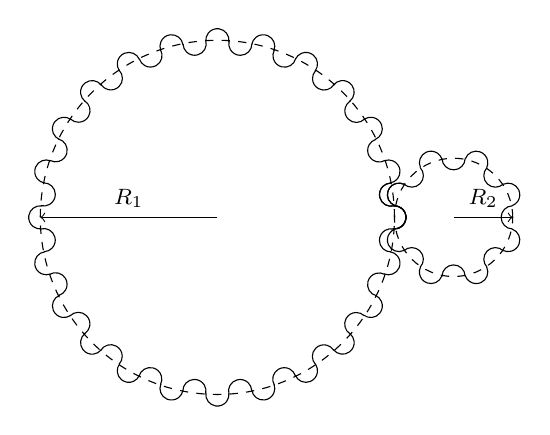
\begin{tikzpicture}[x=1mm,y=1mm]
			\coordinate (m1) at (0,0);
			\coordinate (m2) at (30,0);
			%\path (m1)  + ({22.49085405 * cos(0)},{22.49085405 * sin(0)}) arc[radius = 22.49085405, start angle=0,end angle =360] coordinate[pos=0] (km1) ;
			\draw[dashed] (m1)  + ({22.49085405 * cos(0)},{22.49085405 * sin(0)}) arc[radius = 22.49085405, start angle=0,end angle =360] coordinate[pos={8/360}] (km2) ;
			\draw[dashed] (m2)  + ({7.508037642 * cos(0)},{7.508037642 * sin(0)}) arc[radius = 7.508037642, start angle=0,end angle =360] ;
			%big gear
			\foreach \i in {0,1, ...,24}{
				\begin{scope}[rotate around={\i*15:(m1)}]
				%nach aussen
				\draw (22.49196236,0) + ({1.471832758 * cos(-97.87500000)},{1.471832758 * sin(-97.87500000)}) arc[radius=1.471832758,start angle = -97.87500000,end angle = 95.87500000];
				%nach innen
				\draw ({22.49196236*cos(7.5)},{22.49196236*sin(7.5)}) + ({1.471832758 * cos(-84)},{1.471832758 * sin(-84)}) arc[radius=1.471832758,start angle = -74.37500000,end angle = -268.125];
				\end{scope}
			}
			
			%small gear
			\foreach \i in {0,1, ...,8}{
				\begin{scope}[rotate around={\i*45:(m2)}]
				%nach aussen
				\draw (22.49196236,0) + ({1.471832758 * cos(-88.62500000)},{1.471832758 * sin(-88.62500000)}) arc[radius=1.471832758,start angle = -88.62500000,end angle = 88.62500000];
				%nach innen
				\draw (m2) ++ ({180-45/2}:7.508037642) ++ ({1.471832758 * cos(-110.12500000)},{1.471832758 * sin(-110.12500000)}) arc[radius=1.471832758,start angle = -110.12500000,end angle = -294.875];
				\end{scope}
			}
				
			%radii
			\draw[->] (m1) -- +(-22.49196236,0) node[pos=0.5,above] {\footnotesize$R_1$};
			\draw[->] (m2) -- +(7.508037642,0) node[pos=0.5,above] {\footnotesize$R_2$};		
			\end{tikzpicture}
		\end{figure}
		
		\vfill
		
		% Bottom of the page
		{\large \today\par}
	\end{titlepage}
	\restoregeometry
	
	\thispagestyle{firststyle}

	\newpage
	\tableofcontents
	\thispagestyle{firststyle}
	
	\newpage
	\section{Tooth Profile}
		Since FDM 3d printed gears are weak and therefore torque and transmission efficiency is not as important we are going to use a circular tooth profile. Please note that this profile is not optimal but it makes it incredibly easy to calculate and draw non circular gears. It is sufficient for most 3d printed parts. If this is not suitable for your design take a look at involute gears.\\
		\begin{figure}[!h]
			\centering
%		\begin{tikzpicture}[scale=1]
%			\draw[gray,dashed,thick] (0,0) arc[radius=5cm,start angle=44,end angle =136];
%			\path (0,0) arc[radius=5cm,start angle=44,end angle =136] node[pos=0.5] (A) {};
%			\path (0,0) arc[radius=5cm,start angle=44,end angle =136] node[pos=0.25] (B) {};
%			\path (0,0) arc[radius=5cm,start angle=44,end angle =136] node[pos=0.75] (C) {};
%			\path (0,0) arc[radius=5cm,start angle=44,end angle =136] node[pos=0] (D) {};
%			\path (0,0) arc[radius=5cm,start angle=44,end angle =136] node[pos=1] (E) {};
%			%middle circle:
%			\draw[gray,ultra thick] (A)+(0,1) arc[radius=1cm,start angle=90,end angle =185.73917045];
%			\draw[gray,ultra thick] (A)+(0,1) arc[radius=1cm,start angle=90,end angle =-5.73917045];		
%			\draw[gray,dashed,thick] (A)+(0,-1) arc[radius=1cm,start angle=-90,end angle =-174.2608296];		
%			\draw[gray,dashed,thick] (A)+(0,-1) arc[radius=1cm,start angle=-90,end angle =-5.73917045];
%			
%			%right circle:
%			\draw[gray,dashed,thick] (B)+({cos(-28.73917045)},{sin(-28.73917045)}) arc (-28.73917045:162.73917045:1);
%			\draw[gray,ultra thick] (B)+({cos(-28.73917045)},{sin(-28.73917045)}) arc (-28.73917045:-197.26082955:1);
%			
%			%left circle
%			\draw[gray,dashed,thick] (C)+({cos(17.26082955)},{sin(17.26082955)}) arc (17.26082955:208.73917045:1);
%			\draw[gray,ultra thick] (C)+({cos(17.26082955)},{sin(17.26082955)}) arc (17.26082955:-151.26082955:1);
%			
%			
%			%right most circle:
%			\draw[gray,ultra thick] (D)+({cos(46.73917045)},{sin(46.73917045)}) arc (46.73917045:139.73917045:1);
%			\draw[gray,dashed] (D)+({cos(-134.73917045)},{sin(-134.73917045)}) arc (-134.73917045:-220.26082955:1);
%			
%			%left most circle:
%			\draw[gray,ultra thick] (E)+({cos(39.73917045)},{sin(39.73917045)}) arc (39.73917045:133.73917045:1);
%			\draw[gray,dashed] (E)+({cos(-44.73917045)},{sin(-44.73917045)}) arc (-44.73917045:46.26082955:1);
%			
%			\coordinate (O) at ($(A)+(0,-5)$);
%			
%			\draw[gray,ultra thick,dashed] (O) -- ($(O)!6cm!(D)$);
%			\draw[gray,ultra thick,dashed] (O) -- ($(O)!6cm!(E)$);
%			
%		\end{tikzpicture}
		\begin{tikzpicture}[x=1mm,y=1mm,spy using outlines=
		{circle, magnification=4, connect spies}]
		\draw[dashed] (0,0)  + ({22.49085405 * cos(0)},{22.49085405 * sin(0)}) arc[radius = 22.49085405, start angle=0,end angle =360];
		
			%big gear
			\foreach \i in {0,1, ...,24}{
				\begin{scope}[rotate around={\i*15:(m1)}]
				%nach aussen
				\draw (22.49196236,0) + ({1.471832758 * cos(-97.87500000)},{1.471832758 * sin(-97.87500000)}) arc[radius=1.471832758,start angle = -97.87500000,end angle = 95.87500000];
				%nach innen
				\draw ({22.49196236*cos(7.5)},{22.49196236*sin(7.5)}) + ({1.471832758 * cos(-84)},{1.471832758 * sin(-84)}) arc[radius=1.471832758,start angle = -74.37500000,end angle = -268.125];
				\end{scope}
			}
		\draw[->] (0,0) -- +(-22.49196236,0) node[pos=0.5,above] {\footnotesize$R_1$};
		

		%zoom
		\spy[size=4cm] on (22.49196236,0) in node (zoom) [left] at (70,0);
		\end{tikzpicture}
		\caption{Gear profile construction using circles}
		\end{figure}
		%abbidung close up 3 zaehne
	
	\section{Drawing a Gear}
	Start by drawing the general shape of the gear. As we will see in \cref{non-circular} this can be any convex shape. As an example we will take a look at a circular gear. Then, using a compas, mark points with distance $r$ on the outline of your shape and draw a circle with radius $r$ on every second mark. 
	\begin{figure}[h!]
			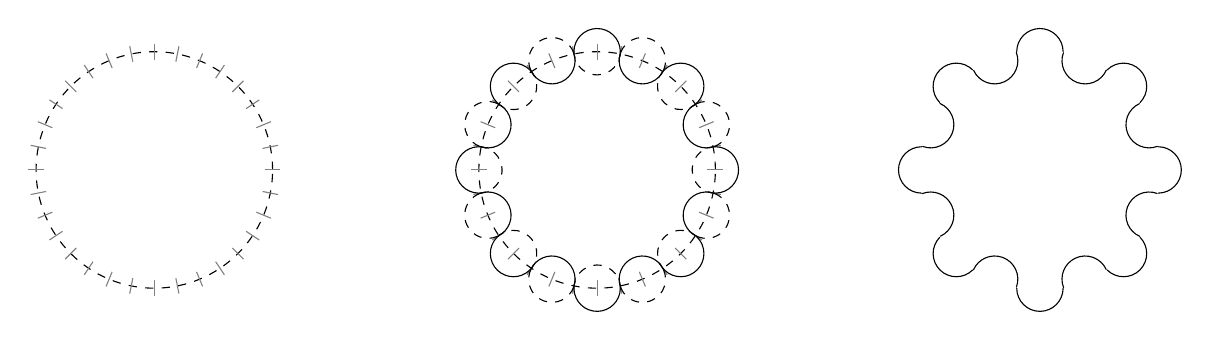
\begin{tikzpicture}[x=1mm,y=1mm,scale = 2]
			\draw[dashed] (0,0) circle[radius = 7.508037642];
			\foreach \i in {0,1,...,31}
			{
				\begin{scope}[rotate=\i*360/32]
				\draw[gray] (7.008037642,0) -- (8.008037642,0);
				\end{scope}
			}
		\begin{scope}[xshift=80]
			\draw[dashed] (0,0) circle[radius = 7.508037642];
			\foreach \i in {0,1,...,31}
			{
				\begin{scope}[rotate=\i*360/32]
				\draw[gray] (7.008037642,0) -- (8.008037642,0);
				\end{scope}
			}
			\foreach \i in {0,1,...,7}
			{
				\begin{scope}[rotate=\i*360/8]
				
				%nach aussen
				\draw (7.508037642,0) + ({1.471832758 * cos(-88.62500000)},{1.471832758 * sin(-88.62500000)}) arc[radius=1.471832758,start angle = -88.62500000,end angle = 88.62500000];
				\draw[dashed] (7.508037642,0) + ({1.471832758 * cos(-88.62500000)},{1.471832758 * sin(-88.62500000)}) arc[radius=1.471832758,start angle = -88.62500000,end angle = -271.375];
				%nach innen
				\draw[dashed] (0,0) ++ ({180-45/2}:7.508037642) ++ ({1.471832758 * cos(-110.12500000)},{1.471832758 * sin(-110.12500000)}) arc[radius=1.471832758,start angle = -110.12500000,end angle = -294.875];
				\draw (0,0) ++ ({180-45/2}:7.508037642) ++ ({1.471832758 * cos(-110.12500000)},{1.471832758 * sin(-110.12500000)}) arc[radius=1.471832758,start angle = -110.12500000,end angle = 66.125];
				
				
				\end{scope}
			}
			\end{scope}
			
			\begin{scope}[xshift=160]
			\foreach \i in {0,1,...,7}
			{
				\begin{scope}[rotate=\i*360/8]
				
				%nach aussen
				\draw[line cap=round] (7.508037642,0) + ({1.471832758 * cos(-89.62500000)},{1.471832758 * sin(-89.62500000)}) arc[radius=1.471832758,start angle = -89.62500000,end angle = 89.62500000];
				%nach innen
				\draw[line cap=round] (0,0) ++ ({180-45/2}:7.508037642) ++ ({1.471832758 * cos(-110.12500000)},{1.471832758 * sin(-110.12500000)}) arc[radius=1.471832758,start angle = -110.12500000,end angle = 66.125];
				
				
				\end{scope}
			}
			\end{scope}
		\end{tikzpicture}
		\caption{Drawing a circular gear}
	\end{figure}
	
	\newpage
	\section{Notation}
	A gear can be represented as a tupel which consists of the gear shape together with the number of teeth, the radius of each tooth, a set containing the centerpoints of each tooth and the centerpoint of the gear itself.
	
	
	\begin{mydefinition}
		A tupel $(\gamma, n, r, (m_i)_{i\in\mathbb{Z}_{2n}}, M)$ where $\gamma:[0,2\pi)\to\mathbb{R}^k$, $k\in\mathbb{N},n\in2\mathbb{N}$, $r\in\mathbb{R}$, $m_i\in\gamma[[0,2\pi)]:d(m_i,m_{i+1})=r$ and $M\in\mathbb{R}^k$ is called a gear. 
	\end{mydefinition}

	If $\gamma$ is a circle we will sometimes replace it with its radius $R\in\mathbb{R}$.
	Furthermore $M$ is defined as point with distance $d(M,\gamma(\varphi)) = ||\gamma(\varphi)||_2, \forall\varphi\in[0,2\pi)$. Since $M$ is defined by $\gamma$ it is not required. However we will only omit $M$ if it is $0$.
	
	
	\begin{mydefinition}
		Two gears are of the same size or shape, if it is possible to map the image of $\gamma_A$ to the image of $\gamma_B$ without changing its size:
		\begin{align}
		\exists\iota: d(\iota(x),\iota(y))=d(x,y)\land\iota(\gamma_A[[0,2\pi)]) = \gamma_B[[0,2\pi)].\label{imp:sim}
		\end{align}
		We call two gears $A$ and $B$ similar and write $A\sim B$ if they are of the same size and
		\begin{gather*}
		n_A=n_B\\
		r_A=r_B\\
		\iota[(m_{A,i})_{i\in\mathbb{Z}_{2n_A}}] = (m_{B,j})_{j\in\mathbb{Z}_{2n_B}}
		\end{gather*}
		where $\iota$ is an isometric function that satisfies \eqref{imp:sim}.
		
	\end{mydefinition}

	\begin{myproof}
		
		
		For this definition to make sense $\sim$ needs to be reflexive, symmetric and transitive.\\
		{ "$A\sim A$":}\par
		Let $\iota$ be the identity.\\
		{ "$A\sim B\implies B\sim A$":}\par
		As $\iota$ is an isometric isomorphism it is bijective and therefore its inverse $\iota^{-1}$ exists. Using $\iota^{-1}$, $B\sim A$.\\
		{ "$A\sim B\land B\sim C\implies A\sim C$":}\par
		The composition of two isometric isomorphisms is an isometric isomorphism and therefore $A\sim C$.
	\end{myproof}
	
	
	\begin{mydefinition}
		Two gears $A$ and $B$ fit together if 
		\begin{align*}
			r_A=r_B.
		\end{align*}
	\end{mydefinition}
	
	
	\section{Calculating Gear and teeth Size}\label{section-gears}
	\subsection{Circular Gears}\label{section-circ}
	Designing a circular gear is straightforward. We start by drawing a circle $K$ with radius $R$. This will be the size of our final gear. We then look for a sequence of smaller circles $(k_i)_{i\in I}$ with radius $r$ such that their center is on $K$, they intersect each other on $K$, they cover $K$ completely and the number of $k_i$ must be even ($|I|=2n : n\in \mathbb{N}$). This is important since the number of teeth has to be a positive integer. 
	
	%abbildung kreise auf dem kreis
	
	
	\begin{mytheorem}\label{theorem-circle}
		Given a circle $K$ with radius $R$ and $n\in\mathbb{N}$, it is possible to find a sequence of $n$ circles $(k_i)_{i\in I}$ with radius $r$ and center $(m_i)_{i\in I}\in K$ such that $|\{x\in K:d(x,m_i)>r,\forall i\in I\}|=0$ and $|\{x\in K:\exists i,j\in I,d(x,m_i)\leq r\land d(x,m_j)\leq r\}| = n$. Where $d(x,y)$ is the distance between $x$ and $y$. Let $\varphi = \frac{2Pi}{n}$ then
		\begin{align}
		R= \frac{r\cdot\cos\left( \frac{\varphi }{4}\right) }{\sin(\frac{\varphi}{2})}.\label{eq:R-r}
		\end{align}
	\end{mytheorem}

	\begin{myproof}
		
		Let $K$ be a circle with radius $R$ and center $(0,0)$ and $n = 2k$, $k\in\mathbb{N}$ we can, using polar coordinates, construct a sequence $(m_i)_{i\in\mathbb{Z}_{2n}}$, $m_i = \left(R,i\cdot\frac{\pi}{n}\text{rad}\right)$ of $2n$ points on $K$. They are evenly spaced and $r\coloneqq d(m_0,m_1)$. We can now construct a sequence $(k_j)_{j\in\mathbb{Z}_n}$of $n$ circles with radius $r$ and center $m_j:j\equiv 0 \Mod 2$. Therefore $\{x\in K:\exists i,j\in \mathbb{Z}_{2n}: d(x,m_{2i})\leq r\land d(x,m_{2j})\leq r\} = \{m_i:i\equiv 1 \Mod 2,i\in\mathbb{Z}_{2n}\}$ and $|\{m_i:i\equiv 1 \Mod 2,i\in\mathbb{Z}_{2n}\}| = n$.
		
		\begin{figure}[h!]
			\centering
			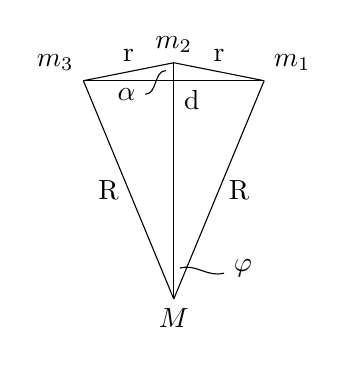
\begin{tikzpicture}[x=1mm,y=1mm,scale = 2]
				\draw (0,0) -- (90:15);
				\draw (0,0) -- (112.5:15) node[pos=0.5,left] {R};
				\draw (0,0) -- (67.5:15) node[pos=0.5,right] {R};
				\draw (90:15) -- (67.5:15) node[pos=0.5,above] {r};
				\draw (90:15) -- (112.5:15) node[pos=0.5,above] {r};
				\draw (67.5:15) -- (112.5:15) node[pos=0.4,below]{d};
				%phi
				\node (phi) at ($(78.75:2) + (4,0) $) {$\varphi$};
				\draw (78.75:2) to[out=15,in=195] (phi);
				%\draw (67.5:3) arc[radius = 3, start angle=67.5,end angle =112.5];
				%alpha
				\node (alpha) at ($(90:15) + (2,-2)  + (-5,0)$) {$\alpha$};
				\draw ($(90:15) + (-0.5,-0.5)$) to[out=180,in=0] (alpha);
				
				\node[below] (M) at (0,0) {$M$};
				\node[above] (m2) at (90:15) {$m_{2}$};
				\node[above right] (m1) at (67.5:15) {$m_{1}$};
				\node[above left] (m3) at (112.5:15) {$m_{3}$};
				
				
			\end{tikzpicture}
		\end{figure}
		
		Let $\alpha\coloneqq\sphericalangle {m_3m_2m_1}$, $\varphi\coloneqq\sphericalangle {m_1Mm_3}$ and $d\coloneqq\overline{m_3m_1}$. Using the inscribed angle theorem\autocite{inscribedangle}, we know that $\alpha=\frac{2\pi - \varphi}{2}$. By drawing a line from $M$ to $m$ we get two right triangles. $\overline{Mm_2}$ also halves  $\varphi$, $\alpha$ and $d$. Thus
		\begin{align}
			\frac{d}{2} = r\cdot\sin\left(\frac{\alpha}{2}\right)\label{eq:d}
		\end{align}
		and
		\begin{align}
			R=\frac{d}{2\sin\left(\frac{\varphi}{2}\right)}.\label{eq:R}
		\end{align}
		By substituting in  $\alpha$ in \cref{eq:d} and using $\cos(x) = \sin(\frac{\pi}{2} - x)$, we see that
		\begin{align}
			R= \frac{r\cdot\cos\left( \frac{\varphi }{4}\right) }{\sin(\frac{\varphi}{2})}.
		\end{align}
		
	\end{myproof}
	

	\subsection{Rectangular Gears}\label{section-rect}
	
	\begin{mytheorem}\label{therem-rectangle}
		%If all four corners of a rectangle $K$ are in $\{m_i:i\in I\}$ and 
		Let $K$ be a rectangle with side lengths of $a$ and $b$. It is possible to find a sequence of circles $(k_i)_{i\in I}$ with the same properties as in \cref{theorem-circle} if $4r\mid a$ and $4r\mid b$. Furthermore all four corners of $K$ are in $\{m_i:i\in I\}$, where $m_i$ is the center of $k_i$.
	\end{mytheorem}

	\begin{myproof}
		It is easy to see that \cref{therem-rectangle} holds true.
	\end{myproof}
	
	
	\subsection{Other Non Circular Gears}\label{non-circular}
	\begin{mytheorem}\label{theorem:non-circular}
		Let $\gamma$ be a simple, closed curve where the enclosed area is convex. $\gamma$ can be used as a gear outline. Furthermore the sequence of circlecenters $\{m_i:i\in I\}$ can be calculated using:\\
		
		\begin{algorithm}[H]
			\SetAlgoLined
			\KwResult{Write here the result }
			I = 2 times number of teeth\;
			\While{While condition}{
				instructions\;
				\eIf{condition}{
					instructions1\;
					instructions2\;
				}{
					instructions3\;
				}
			}
			\caption{Calculating $\{m_i:i\in I\}$}
		\end{algorithm}
	\end{mytheorem}
	
	\subsection{Examples}
	\myexample{Circular gears with given gear ratio and centerdistance}
	Lets say we want a 3:1 gear reduction and the center points of each gear should be 30mm apart. We can now start to build a system of equations:
	\begin{align*}
	R_1 + R_2 &= 30\\
	n_1 &= 3n_2
	\end{align*}
	Where $R_1$ and $R_2$ are the radii of the two gears and $n_1$ and $n_2$ denote the number of teeth on each.	
	Using \cref{eq:R-r} we also know that:
	\begin{align*}
	\varphi_1 &= \frac{2Pi}{n_1}\\
	R_1&= \frac{r*\cos\left( \frac{\varphi_1 }{4}\right) }{\sin(\frac{\varphi_1}{2})}\\
	\varphi_2 &= \frac{2Pi}{n_2}\\
	R_2&= \frac{r*\cos\left( \frac{\varphi_2 }{4}\right) }{\sin(\frac{\varphi_2}{2})}
	\end{align*}
	If we specify the number of teeth on either one of them lets say
	\begin{align*}
	n_2=16.
	\end{align*}
	we can solve the system of equations using wolframalpha, maple or another computerprogram to find a unique solution. In this example we get:
	\begin{align*}
	r &= 1.471832758\\
	R_1 &= 22.49196236\\
	R_2 &= 7.508037642\\
	n_1 &= 48\\
	n_2 &= 16\\
	\varphi_1 &= 0.1308996939\\
	\varphi_2 &= 0.3926990818
	\end{align*}
	If $r$ is too small/large change the number of teeth you specified.
	
	
	\begin{figure}[h!]
		\centering
		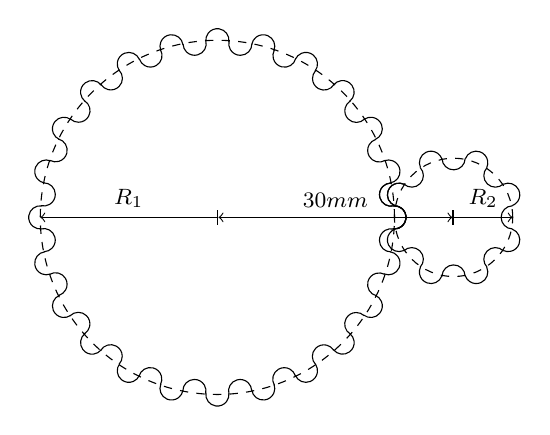
\begin{tikzpicture}[x=1mm,y=1mm]
		\coordinate (m1) at (0,0);
		\coordinate (m2) at (30,0);
		%\path (m1)  + ({22.49085405 * cos(0)},{22.49085405 * sin(0)}) arc[radius = 22.49085405, start angle=0,end angle =360] coordinate[pos=0] (km1) ;
		\draw[dashed] (m1)  + ({22.49085405 * cos(0)},{22.49085405 * sin(0)}) arc[radius = 22.49085405, start angle=0,end angle =360] coordinate[pos={8/360}] (km2) ;
		\draw[dashed] (m2)  + ({7.508037642 * cos(0)},{7.508037642 * sin(0)}) arc[radius = 7.508037642, start angle=0,end angle =360] ;
		%big gear
		\foreach \i in {0,1, ...,24}{
			\begin{scope}[rotate around={\i*15:(m1)}]
			%nach aussen
			\draw (22.49196236,0) + ({1.471832758 * cos(-97.87500000)},{1.471832758 * sin(-97.87500000)}) arc[radius=1.471832758,start angle = -97.87500000,end angle = 95.87500000];
			%nach innen
			\draw ({22.49196236*cos(7.5)},{22.49196236*sin(7.5)}) + ({1.471832758 * cos(-84)},{1.471832758 * sin(-84)}) arc[radius=1.471832758,start angle = -74.37500000,end angle = -268.125];
			\end{scope}
		}
		
		%small gear
		\foreach \i in {0,1, ...,8}{
			\begin{scope}[rotate around={\i*45:(m2)}]
			%nach aussen
			\draw (22.49196236,0) + ({1.471832758 * cos(-88.62500000)},{1.471832758 * sin(-88.62500000)}) arc[radius=1.471832758,start angle = -88.62500000,end angle = 88.62500000];
			%nach innen
			\draw (m2) ++ ({180-45/2}:7.508037642) ++ ({1.471832758 * cos(-110.12500000)},{1.471832758 * sin(-110.12500000)}) arc[radius=1.471832758,start angle = -110.12500000,end angle = -294.875];
			\end{scope}
		}
		
		
		%radii
		\draw[->] (m1) -- +(-22.49196236,0) node[pos=0.5,above] {\footnotesize$R_1$};
		\draw[->] (m2) -- +(7.508037642,0) node[pos=0.5,above] {\footnotesize$R_2$};
		
		\draw[|<->|] (m1) -- +(m2) node[pos=0.5,above] {\footnotesize$30mm$};
		
		
		\end{tikzpicture}
		\caption{Resulting Gears}
	\end{figure}
	
	
	\myexample{Internal ring gear}
	A internal ring gear $K_r$ with outer diameter $D_r = 5$ should be calculated such that a smaller gear $K$ can be used to archive a $5:1$  gear reduction. The two shafts should be $1cm$ apart.\\
	As the two shafts are $15mm$ apart we know that
	\begin{align*}
		R_r-R=15.
	\end{align*}
	Furthermore 
	\begin{align*}
		n_r = 5\cdot n
	\end{align*} 
	to achieve the required $5:1$ ratio.
		Using \cref{eq:R-r} we also know that:
	\begin{align*}
	\varphi_r &= \frac{2Pi}{n_r}\\
	R_r&= \frac{r*\cos\left( \frac{\varphi_r }{4}\right) }{\sin(\frac{\varphi_r}{2})}\\
	\varphi&= \frac{2Pi}{n}\\
	R&= \frac{r*\cos\left( \frac{\varphi }{4}\right) }{\sin(\frac{\varphi}{2})}
	\end{align*}
	If we specify the number of teeth on either one of them lets say
	\begin{align*}
	n=8,
	\end{align*}
	we can solve the system of equations using wolframalpha, maple or another computerprogram to find a unique solution. In this example we get:
	\begin{align*}
	r &= 1.474527091\\
	R_r &= 18.77908826\\
	R &= 3.779088256\\
	n_r &= 40\\
	n &= 8\\
	\varphi_r &= 0.1570796327\\
	\varphi &= 0.7853981635
	\end{align*}
	
	\begin{figure}[h!]
		\centering
		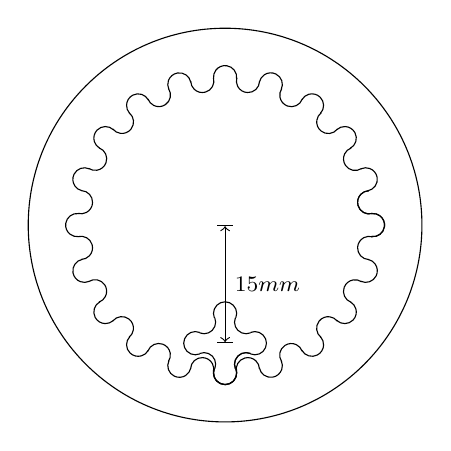
\begin{tikzpicture}[x=1mm,y=1mm]
		\coordinate (m1) at (0,0);
		\coordinate (m2) at (0,-15);
		%\path (m1)  + ({22.49085405 * cos(0)},{22.49085405 * sin(0)}) arc[radius = 22.49085405, start angle=0,end angle =360] coordinate[pos=0] (km1) ;
		%\draw[dashed] (m1)  + ({22.49085405 * cos(0)},{22.49085405 * sin(0)}) arc[radius = 22.49085405, start angle=0,end angle =360] coordinate[pos={8/360}] (km2) ;
		%\draw[dashed] (m2)  + ({7.508037642 * cos(0)},{7.508037642 * sin(0)}) arc[radius = 7.508037642, start angle=0,end angle =360] ;
		
		\draw (m1)  + ({25 * cos(0)},{25 * sin(0)}) arc[radius = 25, start angle=0,end angle =360] ;
		%big gear
		\foreach \i in {0,1, ...,20}{
			\begin{scope}[rotate around={\i*18:(m1)}]
			%nach aussen
			\draw (18.77908826,0) + ({1.4745270918 * cos(-97.87500000)},{1.474527091* sin(-97.87500000)}) arc[radius=1.474527091,start angle = -97.87500000,end angle = 95.87500000];
			%nach innen
			\draw ({18.77908826*cos(9)},{18.77908826*sin(9)}) + ({1.474527091 * cos(-84)},{1.474527091 * sin(-84)}) arc[radius=1.474527091,start angle = -74.37500000,end angle = -268.125];
			\end{scope}
		}
		
		%small gear
		\foreach \i in {0,1, ...,4}{
			\begin{scope}[rotate around={\i*90:(m2)}]
			%nach aussen
			\draw (m2) ++ (-90:3.779088256) ++ ({1.474527091 * cos(-202.5)},{1.474527091 * sin(-202.5)}) arc[radius=1.474527091,start angle = -202.5,end angle = 22.5];
			%nach innen
			\draw (m2) ++ ({-90+45}:3.779088256) ++ ({1.474527091 * cos(67.5)},{1.474527091 * sin(67.5)}) arc[radius=1.474527091,start angle = 67.5,end angle = 202.5];
			\end{scope}
		}
		%radii
		\draw[|<->|] (m1) -- +(m2) node[pos=0.5,right] {\footnotesize$15mm$};
		
		
		\end{tikzpicture}
		\caption{Resulting internal ring gear}
	\end{figure}
	
	
	\myexample{Planetary gears (epicyclic gear train)}
	
	\myexample{Rectangular gear with given tooth size $r$}
	
	\myexample{Rectangular and circular gears with given gear ratio and centerdistance}
	
	
	
	
	
	
	\newpage
	\section{Rack and Pinion}\label{section-rack}
	In order to translate linear motion to rotation and vice versa a rack and pinion can be used. As seen in \cref{section-gears} it is possible to calculate and draw a gearprofile.
	
	
	\begin{figure}[h!]
		\centering
		\begin{tikzpicture}[x=1mm,y=1mm]
		\coordinate (m1) at (0,0);
		%radius = 22.49196236
		%big gear
		\foreach \i in {0,1, ...,24}{
			\begin{scope}[rotate around={\i*15:(m1)}]
			%nach aussen
			\draw (22.49196236,0) + ({1.471832758 * cos(-97.87500000)},{1.471832758 * sin(-97.87500000)}) arc[radius=1.471832758,start angle = -97.87500000,end angle = 95.87500000];
			%nach innen
			\draw ({22.49196236*cos(7.5)},{22.49196236*sin(7.5)}) + ({1.471832758 * cos(-84)},{1.471832758 * sin(-84)}) arc[radius=1.471832758,start angle = -74.37500000,end angle = -268.125];
			\end{scope}
		}
	
		\draw (-51.51414653,-32.49196236) -- (48.570481014,-32.49196236);
		\foreach \i in {0,1, ...,16}{
			\draw ({-51.51414653+1.471832758 + 4*1.471832758*\i},-22.49196236) + ({1.471832758 * cos(0)},{1.471832758 * sin(0)}) arc[radius=1.471832758,start angle = 0,end angle = 180];
			\draw ({-51.51414653+1.471832758 + 2*1.471832758 + 4*1.471832758*\i},-22.49196236) + ({1.471832758 * cos(0)},{1.471832758 * sin(0)}) arc[radius=1.471832758,start angle = 0,end angle = -180];
		}
%		\draw ({-51.51414653+1.471832758 + 4*1.471832758*17},-22.49196236) + ({1.471832758 * cos(0)},{1.471832758 * sin(0)}) arc[radius=1.471832758,start angle = 0,end angle = 180];
		
		\draw (-51.51414653,-32.49196236) to[out=135,in=-45] (-51.51414653,-22.49196236);
		\draw (48.570481014,-32.49196236) to[out=135,in=-45] (48.570481014,-22.49196236);
		
		%arrows:
		\draw[<->] (135:10) to[out=45,in=135] (45:10);
		\draw[<->] (-10,-27.49196236) to (10,-27.49196236);
		
		\end{tikzpicture}
		\caption{Rack and Pinion}
	\end{figure}
	
	
	
	
	\subsection{Constant rotational Speed}
	\begin{mytheorem}
		Let $K$ be a circular gear with not moving center $M$ and $R$ a corresponding rack. There exists a homomorphism $\Psi$ such that $\Psi(s) = \varphi$, where $s$ is the distance $R$ is moved and $\varphi$  the angle $K$ is rotated around $M$. If $R$ is moved at a constant speed, the rotational speed of $K$ will be constant.
	\end{mytheorem}

	\begin{myproof}
		Assuming there is no play in this system $K$ can be viewed as a circle with radius $r$ and the rack $R$ as a tangent line. The length of an arc can be calculated using
		\begin{align*}
			l=r\cdot \varphi
		\end{align*}
		and therefore
		\begin{align*}
			\varphi=\frac{l}{r}.
		\end{align*}
		Since there is no play, the length $l$ of the arc will be equal to the distance $s$, $R$ was moved and 
		\begin{align*}
			\Psi(s) = \frac{s}{r}.
		\end{align*}
		It is easy to see that $\Psi(\lambda\cdot s) = \lambda\cdot\Psi(s)$. As $\Psi$ is a composition of continuous functions it is continuous. \\
		\\
		If $R$ is moving with constant speed $v(t)=\frac{s(t)}{t}=s(1)$, $v'=0$. The rotational speed of $K$, $\omega(t)=\frac{\varphi}{t}$ can be calculated using $\Psi$.
		\begin{align*}
			\omega(t)&= \frac{\Psi(s(t))}{t} = \frac{t\cdot\Psi(s(1))}{t} = \Psi(s(1)) = \Psi(v(t))\\
		\end{align*}
		As $v$ is constant so is $\Psi(v)$ and thus $\omega$ is constant.
		
		%ABSOLUT FALSCH!!!!
		%psi(c1) = c2 ist die richtige begruendung
	\end{myproof}
	
	\subsection{Non-constant rotational Speed}
	If a non-circular gear is used as a pinion and a rack is made in a way that the center of the gear does not move the resulting rotational speed will be non constant. This behavior can be used to calculate a special gear shape such that the rotational speed follows a given curve. Leading to the following theorem:\\
	
	\begin{mytheorem}
		Given a periodic, continuous function $f$. If $\gamma''(\varphi)\leq K''(\varphi)$ where
		\begin{align}
			\gamma(\varphi)= 
			\begin{pmatrix}
				\frac{1}{f(\varphi)}\cos(\varphi)\\
				\frac{1}{f(\varphi)}\sin(\varphi)
			\end{pmatrix},
		\end{align}
		$\gamma$ will be simple, closed and the enclosed area will be convex. $\gamma$ can therefore be used as a gear outline. Furthermore, if a fitting rack moves with constant speed $c$, the rotational speed of this gear will be $cf(\varphi)$.
	\end{mytheorem}

\begin{myproof}
	
\end{myproof}
	\subsection{Non-constant shaft position}
	If it is necessary that the shaft rotates and changes position a control cam can be used (\cref{fig:shaftposition}). By restricting the shaft position in the x direction it will follow the racks shape if they stay in contact. If no rotation is required a control cam in the required shape should be used on its own.
	
	
	
	
		\begin{figure}[h!]
		\centering
		\begin{tikzpicture}[x=1mm,y=1mm]
		\coordinate (m2) at (0,0);
		%radius = 22.49196236
		%small gear
		\foreach \i in {0,1, ...,8}{
			\begin{scope}[rotate around={\i*45:(m2)}]
			%nach aussen
			\draw (-7.508037642,0) + ({1.471832758 * cos(-88.62500000)},{1.471832758 * sin(-88.62500000)}) arc[radius=1.471832758,start angle = -88.62500000,end angle = 88.62500000];
			%nach innen
			\draw (m2) ++ ({180-45/2}:7.508037642) ++ ({1.471832758 * cos(-110.12500000)},{1.471832758 * sin(-110.12500000)}) arc[radius=1.471832758,start angle = -110.12500000,end angle = -294.875];
			\end{scope}
		}
		
		%rack
		\draw (-51.51414653,-32.49196236) -- (48.570481014,-32.49196236);
%		\foreach \i in {0,1, ...,16}{
%			\draw ({-51.51414653+1.471832758 + 4*1.471832758*\i},-22.49196236) + ({1.471832758 * cos(0)},{1.471832758 * sin(0)}) arc[radius=1.471832758,start angle = 0,end angle = 180];
%			\draw ({-51.51414653+1.471832758 + 2*1.471832758 + 4*1.471832758*\i},-22.49196236) + ({1.471832758 * cos(0)},{1.471832758 * sin(0)}) arc[radius=1.471832758,start angle = 0,end angle = -180];
%		}
		
		\draw[domain=-51.51414653:48.570481014,smooth,variable=\x,blue] plot ({\x},{5*sin(\x*5) -18.0});
		
		
		\draw (-51.51414653,-32.49196236) to[out=135,in=-45] (-51.51414653,-13.0);
		\draw (48.570481014,-32.49196236) to[out=135,in=-45] (48.570481014,-22.49196236);
		
		%arrows:
		\draw[<->] (135:10) to[out=45,in=135] (45:10);
		\draw[<->] (-10,-27.49196236) to (10,-27.49196236);
		
		\end{tikzpicture}
		\caption{Rack and Pinion}\label{fig:shaftposition}
	\end{figure}

	\begin{mytheorem}
		Let $K$ be a circular gear with radius $r$ and center $m$ where $m_x$ is constant and $f\in C^2([0,2\pi))$ with $|f''(\varphi)| < |K''(\varphi)|$. $f$ can be used as an outline for a rack $R$ and $m_y$ will follow the curve $f+c,c\in\mathbb{R}$.
	\end{mytheorem}\label{theorem:shaft-pos}

	\begin{myproof}
		Using \cref{theorem:non-circular} it is possible to calculate a gear profile for $K$ and $R$. Since $K$ is circular and always touching $R$, the distance between $m$ and $R$ is $r$. It is easy to see that $|f''(\varphi)| < |K''(\varphi)|$ implies that $K$ is touching $R$ in no more than one point. Thus $m_y = f(\varphi) + r + c$ where $c$ depends on the total thickness of $R$. A proper proof is omitted since it is easy to see that \cref{theorem:shaft-pos} holds true.
	\end{myproof}
	
	
	
	
	\subsection{Examples}
	\myexample{Shaft following a Sinus(t) curve}
	We want a gear such that the shaft is following a $\sin(t)$ curve. We know that $\sin(t)$ is a $2\pi$ periodic function with $\sin(t)>0,t\in(0,\pi)$ and $\sin(t)<0,t\in(\pi,2\pi)$. As seen in \cref{rack} this will result in a non convex gear shape. To use the method described in \cref{non-circular} we need a new function $g(t):=sin(t)+|min(sin[0,2\pi])|$. Thus $g(t)\geq0,t\in(0,2\pi)$ resulting in a convex gear shape. However the shaft will now follow $g(t)$ and not $\sin(t)$. Therefore we need to offset both the rack and pinion by $|min(sin[0,2\pi])|$.\\
	We can now start by choosing a minimum radius $R:=5$ for the gear. \\
	\myexample{cos(t)}
	
	
	
	\newpage
	\printbibliography
	\newpage
	\listoffigures
	\thispagestyle{firststyle}
	\listoftables
	\thispagestyle{firststyle}
	
	\newpage
	\appendix
	\newpage
	
	
\end{document}

